\section{Legal Language Models and Benchmarks (2020--2023)}
\label{sec:lm2023}

Two years after \citet{zhong2018}, the field's center of gravity shifted again. By 2020, large
pretrained language models had become capable enough that researchers could adapt a general-purpose
model to a new domain instead of building one from scratch for every task. This section follows how
the field first connected that capability to external evidence, then adapted it specifically to
legal text, then evaluated it systematically, all within a four-year window.

\subsection{2020: connecting generation to retrieved evidence, outside the legal domain}

The most consequential development of this period, for everything that follows in this survey, was
not legal at all when it first appeared. \citet{lewis2020} introduced retrieval-augmented generation
(RAG): instead of relying only on knowledge encoded in a model's parameters, a RAG system retrieves
external documents at inference time and conditions its generated output on them.
Figure~\ref{fig:lewis-rag} summarizes their architecture.

% The end-to-end retrieval-augmented generation (RAG) architecture of Lewis et al. (2020).
\begin{figure*}[t]
\centering
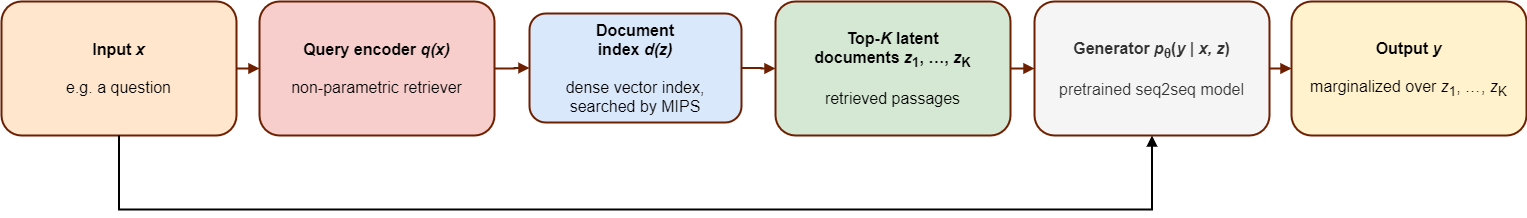
\includegraphics[width=\textwidth]{images/rag_original_architecture.png}
\caption{The end-to-end retrieval-augmented generation (RAG) architecture of
\citet{lewis2020}, redrawn here for discussion. A non-parametric retriever ($q(x)$ over a dense
document index $d(z)$, searched with Maximum Inner Product Search) returns the top-$K$ passages
for an input $x$; a parametric seq2seq generator then conditions on both $x$ and each retrieved
passage and the final output $y$ is marginalized over the retrieved set. This general-domain
architecture, not originally designed for law, is the direct ancestor of every legal RAG pipeline
discussed in the remainder of this survey.}
\label{fig:lewis-rag}
\end{figure*}


A non-parametric retriever, built from a query encoder and a dense document index searched with
Maximum Inner Product Search, returns the top-$K$ passages for an input, and a parametric seq2seq
generator then conditions on the input and each retrieved passage, with the final output
marginalizing over the retrieved set. Lewis et al.\ reported that this architecture improved
performance on knowledge-intensive, open-domain tasks, producing answers that were more specific and
better supported than generation from parameters alone. We introduce RAG here, at its true
publication date and in its original, general-purpose form, for the same reason we introduced
Reciprocal Rank Fusion in Section~\ref{sec:foundations}: researchers did not design it for law, and
this survey will not credit it as though they had. Its legal application came later, as a separate
development this survey reaches in Section~\ref{sec:rag2024}.

In the same year, two further developments addressed complementary problems. \citet{chalkidis2020}
introduced \textbf{LEGAL-BERT}, testing three strategies for adapting the BERT architecture to legal
text: using the original pretrained model as is, continuing its pretraining on legal corpora, or
pretraining a new model from scratch on legal text. They released a family of legal language models
for later research, illustrated in Figure~\ref{fig:legalbert}. The underlying principle is simple:
if a model has to process legal documents, its training should expose it to the language and
terminology those documents use. Readers should not treat LEGAL-BERT as a complete legal reasoning
system, though, since it provides learned language representations for specific NLP tasks; it does
not determine which authority governs a dispute, and it does not confirm that the cited text
supports a generated conclusion.

% Original diagram summarizing the three BERT adaptation strategies of Chalkidis et al.
% (2020), "LEGAL-BERT: The Muppets Straight out of Law School" (Findings of EMNLP 2020),
% Figure 1. Redrawn in this paper's own visual style; cited in the caption and surrounding text.
\begin{figure*}[t]
\centering
\resizebox{\textwidth}{!}{%
\begin{tikzpicture}[
  font=\scriptsize,
  lbl/.style={font=\scriptsize\bfseries, align=center},
  stg/.style={draw, thick, rounded corners=2pt, align=center, text width=3.0cm,
              minimum height=12mm, inner sep=2pt},
  rowlbl/.style={font=\small\bfseries, align=left, anchor=east}]

  \node[lbl] at (2.5,1.2)  {Pre-train};
  \node[lbl] at (6.5,1.2)  {Adapt};
  \node[lbl] at (10.5,1.2) {Fine-tune};

  % row (a) BERT-BASE
  \node[rowlbl] at (-0.3,0) {(a) BERT-BASE};
  \node[stg, fill=orange!25, draw=orange!70] (a1) at (2.5,0) {Generic Corpora};
  \node[stg, fill=blue!20, draw=blue!60]     (a3) at (10.5,0) {Task Data};
  \draw[-{Latex[length=2.4mm]}, line width=0.9pt] (a1) -- (a3);

  % row (b) LEGAL-BERT-FP
  \node[rowlbl] at (-0.3,-1.6) {(b) LEGAL-BERT-FP};
  \node[stg, fill=orange!25, draw=orange!70] (b1) at (2.5,-1.6) {Generic Corpora};
  \node[stg, fill=cyan!20, draw=cyan!60]     (b2) at (6.5,-1.6) {Domain Corpora};
  \node[stg, fill=blue!20, draw=blue!60]     (b3) at (10.5,-1.6) {Task Data};
  \draw[-{Latex[length=2.4mm]}, line width=0.9pt] (b1) -- (b2);
  \draw[-{Latex[length=2.4mm]}, line width=0.9pt] (b2) -- (b3);

  % row (c) LEGAL-BERT-SC
  \node[rowlbl] at (-0.3,-3.2) {(c) LEGAL-BERT-SC};
  \node[stg, fill=cyan!20, draw=cyan!60]     (c2) at (2.5,-3.2) {Domain Corpora};
  \node[stg, fill=blue!20, draw=blue!60]     (c3) at (10.5,-3.2) {Task Data};
  \draw[-{Latex[length=2.4mm]}, line width=0.9pt] (c2) -- (c3);

\end{tikzpicture}}
\caption{The three strategies for adapting BERT to a downstream legal NLP task, from
\citet{chalkidis2020}, redrawn here for discussion. (a) BERT-BASE uses the original pretrained
model as-is and fine-tunes directly on task data; (b) LEGAL-BERT-FP further pretrains BERT on
domain-specific (legal) corpora before fine-tuning; (c) LEGAL-BERT-SC pretrains a new model from
scratch on domain-specific corpora. All three alternatives share a final fine-tuning step on the
task data.}
\label{fig:legalbert}
\end{figure*}


Separately, \citet{sovrano2020} built legal knowledge graphs for question answering by combining
open knowledge-extraction tools with NLP techniques. This extended the structured-representation
idea legal ontologies first raised in Section~\ref{sec:foundations} into a form that could support
graph-based retrieval, a technique this survey returns to in Section~\ref{sec:rag2024}.

\subsection{2021: a harder benchmark for legal pretraining}

The following year, \citet{zheng2021} introduced \textbf{CaseHOLD}, a dataset built from the holding
statements of US case law. The authors designed it specifically to test whether domain-specific
pretraining measurably helps on a genuinely difficult legal task, identifying the correct holding
for a citing context, rather than on easier, more generic classification problems. Their results
showed that domain pretraining's benefit depends on the task: it helped substantially on CaseHOLD,
more than on easier legal benchmarks. That sharpened the question the next two years of research
would take up directly: which legal tasks, specifically, need legal language understanding, and how
should researchers measure that systematically?

\subsection{2022: systematic evaluation, and a field looking back on itself}

Five developments from 2022, taken in sequence, answered that question from different angles.
\citet{chalkidis2022} introduced \textbf{LexGLUE}, a benchmark that brings together multiple legal
language-understanding datasets, including CaseHOLD, in one standardized evaluation setting, and
reported that legal-oriented models consistently outperformed general-purpose models across its
tasks. Strong LexGLUE results show legal language understanding on its constituent datasets, but
they do not, by themselves, show that a system can retrieve the correct authority for a new question
or verify a citation. \citet{zhu2022} then applied the knowledge-graph idea \citet{sovrano2020} had
introduced two years earlier to multilevel legal and regulatory frameworks, designing a
knowledge-graph retrieval system over latent semantic indexing for legal and regulatory text. This
extended graph-based legal retrieval from question answering toward a more general retrieval
architecture. \citet{sansone2022} then surveyed the state of the art in legal information retrieval
directly, pulling the lexical and early semantic retrieval methods this survey introduced in
Sections~\ref{sec:foundations} and~\ref{sec:outcomes} into a systematic account of the open problems in the field. \citet{rabelo2022}
reported on the 2021 edition of the Competition on Legal Information Extraction and Entailment
(COLIEE), an annually recurring benchmark drawn from the Japanese Civil Code and Japanese Bar
Examination questions; this competition evaluates legal information retrieval and entailment
jointly, and this survey revisits later editions of it in Sections~\ref{sec:rag2024} and~\ref{sec:2026}
as the field publishes them. Finally, and apart from these four technical contributions,
\citet{villata2022}, writing with Kevin Ashley himself three decades after HYPO, reviewed the third
decade of the \emph{Artificial Intelligence and Law} journal. They identified the same shift this
survey has just traced in its own narrative: a move away from the symbolic, rule-based, and
case-based techniques that opened this survey, toward machine-learning approaches applied to
natural-language legal text. A leading founder of the field, reflecting on thirty years of his own
discipline, described exactly the transition this survey narrates independently, which gives us a
useful external confirmation that the chronology presented here reflects the field's actual
development, not just a convenient organizing device we chose for this paper.

\subsection{2023: legal reasoning as a benchmark, in its own right}

\citet{guha2023} extended the evaluation question CaseHOLD had raised and LexGLUE had answered
toward a broader target: legal \emph{reasoning}, not only legal language understanding.
\textbf{LegalBench} is a collaboratively built benchmark of 162 tasks spanning six types of legal
reasoning; legal professionals helped build it, and the authors used it to evaluate twenty
open-source and commercial LLMs. LegalBench and LexGLUE are complementary rather than competing:
LexGLUE standardizes legal language-understanding evaluation, while LegalBench targets a broader
range of reasoning tasks, and neither one solves the problem of grounding a generated answer in a
correct, current, and authoritative legal source. In the same year, \citet{goebel2023} summarized
the 2023 edition of the same COLIEE competition \citet{rabelo2022} had reported on the year before,
a series this survey revisits again in Sections~\ref{sec:rag2024} and~\ref{sec:2026} as later
editions appear.

Table~\ref{tab:lmdev} summarizes what this four-year period enabled and what it left unresolved.

\begin{table*}[tp]
\centering
\caption{Major developments in legal language models and evaluation, in chronological order (2020--2023).}
\label{tab:lmdev}
\footnotesize
\setlength{\tabcolsep}{5pt}
\renewcommand{\arraystretch}{1.25}
\begin{tabularx}{\textwidth}{>{\raggedright\arraybackslash}p{1.1cm} >{\raggedright\arraybackslash}p{2.6cm} >{\raggedright\arraybackslash}X >{\raggedright\arraybackslash}X}
\toprule
\textbf{Year} & \textbf{Development} & \textbf{What it enabled} & \textbf{What it did not establish} \\
\midrule
2020 & RAG \citep{lewis2020} & A general architecture for conditioning generation on retrieved external evidence. & Any legal content, grounding, or verification specific to law. \\
2020 & LEGAL-BERT \citep{chalkidis2020} & Reusable pretrained representations for legal NLP research. & End-to-end legal reasoning or guaranteed factual correctness. \\
2021 & CaseHOLD \citep{zheng2021} & A genuinely hard test of domain pretraining on US case holdings. & That domain pretraining helps equally on every legal task. \\
2022 & LexGLUE \citep{chalkidis2022} & Standardized comparison of general-purpose and legal-oriented models. & Reliable retrieval and generation of evidence-grounded answers. \\
2023 & LegalBench \citep{guha2023} & Direct investigation of LLM capability on 162 legal reasoning tasks. & Universal competence across jurisdictions or legal practice settings. \\
\bottomrule
\end{tabularx}
\end{table*}

Three limitations carried forward out of this period, and they define the problem the rest of this
survey addresses. Learned representations do not guarantee access to authoritative evidence, since
no one can assume a model knows whether a statute has since been amended. Benchmark success is not
the same as legal reliability, since classification accuracy does not establish that every claim in
a response is factually supported. And legal context remains essential, since a model may process a
paragraph accurately while missing the exception or amendment that changes its meaning. These are
exactly the limitations that, starting in 2024, pushed the field to increasingly combine its
language models with the retrieval-augmented generation architecture \citet{lewis2020} had
introduced four years earlier for an entirely different domain.
